\lezione{21}{24.05.2017}

\section{Leggi condizionate}
\label{section-leggi-condizionate}
In questo capitolo riprenderemo il concetto di \emph{probabilità condizionata} giustificandone esistenza e unicità, che prima erano date per scontate.
Saranno riformulate le definizioni già viste, passando dal linguaggio degli eventi a quello delle variabili aleatorie ed estendendole a una trattazione più astratta e generale.
Analizzando alcuni casi particolari, ritroveremo quanto precedentemente osservato su densità e probabilità condizionate.
\smallskip
\begin{defn}
	\index{legge!condizionata}
  Siano $(\Omega, \Ac, \PP)$ spazio di probabilità, $(E, \Ec), (F, \Fc)$ spazi misurabili, $X: \Omega \to E, \ Y: \Omega \to F$ VA.

  La funzione $Q: E \times \Fc \to [0, 1]$ è una \textbf{legge condizionata} (o distribuzione condizionata) se:
  \begin{enumerate}
    \item $\forall B \in \Fc$ fissato, la funzione $Q(\, \bigcdot \, , B): E \to [0, 1]$ è $\Ec$-misurabile;
    \item $\forall x \in E$ fissato, la funzione $Q(x, \, \bigcdot \,): \Fc \to [0, 1]$ è una probabilità;
    \item $\forall A \in \Ec, \ \forall B \in \Fc, \enspace \PP(X \in A, Y \in B) = \bigintsss_E \Ind_A(x) \, Q(x, B) \, P^X(\dx)$.
  \end{enumerate}
\end{defn}

Notiamo che il punto (3) è una generalizzazione al caso continuo della formula delle probabilità totali. Perché l'integrale abbia senso, è necessario che sia rispettata l'ipotesi di misurabilità di cui al punto (1).

Il concetto di \emph{legge condizionata}, pur diverso nella definizione, è analogo a quello di probabilità condizionata che avevamo già visto a suo tempo. \\ Intuitivamente scriveremo: $P^{Y|X}(B|x) = \PP(Y \in B | X = x) \eqqcolon Q(x|B)$

Vale inoltre la seguente proprietà, simile alla definizione di probabilità condizionata vista a pagina \pageref{prob-condizionata} del capitolo 2:
$$P^{Y|X}(y \,| x) = \PP(Y = y \,| X = x) = \dfrac {\PP(Y=y, X=x)} {\PP(X=x)} = \dfrac {P^{(X, Y)}(x, y)} {P^X(x)}$$

Si può dimostrare che l'\emph{esistenza} di $Q$ è garantita nel caso particolare di $(F, \Fc) = (\RR^n, \Bc^n)$.
Non ci addentriamo nelle ipotesi aggiuntive richieste su uno spazio misurabile $(F, \Fc)$ generico.
Vale inoltre l'\emph{unicità} di $Q$ a meno di insiemi a misura nulla; ovvero, se $Q$ e $\widetilde{Q}$ sono due leggi condizionate di $Y$ data $X$, allora è vero che, $\forall B \in \Fc, \ Q(x, B) = \widetilde Q(x, B)$ quasi certamente rispetto a $P^X$ (scritto anche come $P^X$-qc).

\subsection{Valori attesi rispetto a una legge condizionata}

Sia $(F, \Fc) = (\RR^n, \Bc^n)$.
Introduciamo alcune grandezze delle leggi condizionate, le cui definizioni sono omologhe a quelle viste per le normali distribuzioni.
\begin{defn}
	\index{valore atteso!condizionato}
	\index{varianza!condizionata}
	\index{covarianza!condizionata}
  Il \textbf{valore atteso condizionato} di $Y_k$ data $X$ è definito come:
    $$\EE[Y_k|X=x] = m(x) \coloneqq \int_{\RR^n} y \, Q(x, \dy)$$
  La \textbf{varianza condizionata} di $Y_k$ data $X$ è definita come:
    $$Var(Y_k|X=x) = q^2(x) \coloneqq \int_{\RR^n} \left(y - \EE \left[Y_k|X=x \right] \right)^2 \, Q(x, \dy)$$
  La \textbf{covarianza condizionata} di $Y_k$ e $Y_l$ data $X$ è definita come:
    $$Cov(Y_k, Y_l|X=x) = \int_{\RR^n} \left(y_k - \EE\left[Y_k|X=x\right]\right) \, \left(y_l - \EE\left[Y_l|X=x\right]\right) \, Q(x, \dy)$$
\end{defn}

Nel caso discreto le definizioni sono del tutto simili:
\begin{itemize}
  \item $\EE\left[Y|X=x\right] = \sum\limits_{y \in S_Y} y \, p_{Y|X}(y|x)$
  \item $Var\left[Y|X=x\right] = \sum\limits_{y \in S_Y} \left(y - \EE\left[Y|X=x\right]\right)^2 \, p_{Y|X}(y|x)$
  \item $\EE\left[h(Y)|X=x\right] = \sum\limits_{y \in S_Y} h(y) p_{Y|X}(y|x)$
\end{itemize}

\subsubsection{Indipendenza}

\begin{prop}
  $X$ e $Y$ sono indipendenti se e solo se $P^{Y|X}(B|x) = P^{Y}(B)$ qc rispetto a $P^X$, $\forall B \in \Fc$.
\end{prop}
La condizione è simile, \emph{mutatis mutandis}\footnote{``Con le opportune modifiche'', dice Wikipedia. Verri non vi ha proprio insegnato niente?}, a una delle proprietà della probabilità condizionata: una VA è indipendente da un'altra se e solo se la sua legge rimane identica dopo il condizionamento. L'unica differenza è il linguaggio utilizzato, prima quello di indipendenza di eventi e di probabilità, ora quello di indipendenza di VA e di legge.
\medskip

\begin{ese}
Dato $Y = h(X)$ con $h: E \to F$ misurabile, allora $P^{Y|X}(B|x) = \Ind_B(h(x)) = \delta_{h(x)}(B)$.
\end{ese}
\medskip

\begin{ese}[paradosso di Borel]
	\index{Borel!paradosso di}
Siano $X, Y$ VA indipendenti di legge $\Ec(\lambda)$, con $\lambda > 0$. \\
Sia inoltre $Z = \frac {X - 1} Y$. \\
In tal caso, $Y | X = 1 \not\sim Y | Z = 0$, ovvero, in termini di leggi condizionate, $P^{Y|X}(\, \bigcdot \, | 1) \not\sim P^{Y|Z}(\, \bigcdot \,|0)$. \\
Questo problema sorge dal fatto che l'evento $A = (X = 1) = (Z = 0)$ abbia probabilità nulla, e che dunque le seguenti espressioni non sono ben definite: $$P^{Y|X}(y | 1) = \frac {P^{(X, Y)}(1, y)} {P^X(1)}, \qquad P^{Y|Z}(y | 0) = \frac {P^{(Z, Y)}(0, y)} {P^Z(0)}$$
Pertanto, quando d'ora in avanti ci si riferirà ad eventi della forma $(Z=0)$, li si penserà sempre come ottenuti dal limite per $\varepsilon \to 0$ degli eventi della forma $(-\varepsilon < Z < \varepsilon)$, che sono eventi non improbabili e quindi non generano ambiguità.
\end{ese}
\begin{figure}[H]
  \tikzset{
    hatch distance/.store in=\hatchdistance,
    hatch distance=10pt,
    hatch thickness/.store in=\hatchthickness,
    hatch thickness=2pt
  }

  \centering
  \begin{tikzpicture}
  \begin{axis}[
    axis lines = middle,
    ylabel = $Y$,
    xlabel = $X$,
    width=0.9\textwidth,
    height=0.5\textwidth,
    yticklabels={,,},
    xticklabels={,,},
		every axis y label/.style={at={(current axis.above origin)},anchor=north east}
  ]

  \fill[mark=none,
    domain=-5:1,
    samples=100,
    pattern=flexible hatch,
    hatch distance=5pt,
    hatch thickness=0.5pt,
    draw=lightblue,
    pattern color=lightblue] (axis cs:1,0) -- (axis cs:1.75,6) -- (axis cs:0.25,6) -- (axis cs:1,0);

  \addplot [
    domain=-1:1,
    samples=500,
    color=black,
    line width=0.2mm
    ]
    {-2*(x-1)};

  \addplot [
    domain=1:3,
    samples=500,
    color=black,
    line width=0.2mm
    ]
    {2*(x-1)};

  \addplot [
    domain=0:1,
    samples=500,
    color=black,
    line width=0.2mm
    ]
    {-4*(x-1)};

  \addplot [
    domain=1:2,
    samples=500,
    color=black,
    line width=0.2mm
    ]
    {4*(x-1)};

  \addplot [
    domain=0.5:1,
    samples=500,
    color=black,
    line width=0.2mm
    ]
    {-8*(x-1)};

  \addplot [
    domain=1:1.5,
    samples=500,
    color=black,
    line width=0.2mm
    ]
    {8*(x-1)};

	\draw[line width=0.3mm, dashed] (axis cs:1,0) -- (axis cs: 1,12);

  \node at (axis cs:1.1,2.5) {} edge[<-, line width=0.5mm, color=lightblue, looseness=1, bend left=20]  (axis cs:2.3, 1.5) ;
  \node at (axis cs:0.9,2.5) {} edge[<-, line width=0.5mm, color=lightblue, looseness=1, bend right=20]  (axis cs:-0.3, 1.5) ;
  \node[color=lightblue] at (axis cs:1.75,1.95) {\large{$\bm{\varepsilon \!\downarrow}$}};
  \node[color=lightblue] at (axis cs:0.25,1.95) {\large{$\bm{\varepsilon \!\downarrow}$}};

  \addplot [draw=none, forget plot] coordinates {(0,-0.35)};
  \draw[line width=0.60mm, color=white] (axis cs:0,-1) -- (axis cs: 0, -0.01);
  \node[below] at (axis cs:1,0) {$1$};

  \end{axis}
  \end{tikzpicture}
  \caption{la retta $(Z=0)$ ottenuta come limite dei coni $(-\varepsilon < Z < \varepsilon)$}
\end{figure}

\vskip\bigskipamount
\begin{nb}
  Come già notato, vale $P^{(X, Y)}(x, y) = P^{Y|X}(y|x) \cdot P^X(X)$. \\
  Dunque conoscere $P^{(X, Y)}$ \emph{(probabilità congiunta)} equivale a conoscere $P^X$ \emph{(probabilità marginale)} e $P^{Y|X}(\, \bigcdot \, | x)$ \emph{(probabilità condizionata)}.
\end{nb}
Occupiamoci allora di legare la probabilità congiunta alla probabilità condizionata in alcuni casi di particolare rilevanza.

\subsection{Casi discreti}

\subsubsection{Con due variabili aleatorie}
\begin{ese}\label{ese-dadi-monete-teste}
  Si lanci un dado, seguito dal lancio di un numero di monete pari al risultato del dado.
  Qual è la legge congiunta del numero di teste e del risultato del dado?

  Definiamo le VA discrete $D$, risultato del dado, e $T$, numero di teste. Ovviamente $D \sim U(\{ 1, \dots, 6\})$.
  Scriviamo $T$ come legge condizionata: come già noto, si ha $T | D=n \sim B \left( n, \dfrac 1 2 \right)$.
  I supporti delle due VA sono rispettivamente $S_D = \{ 1, \dots, 6 \}$ e $S_T = \{ 0, \dots, 6 \}$. Il supporto del vettore aleatorio sarà dunque trapezoidale.

  \begin{figure}[H]
    \centering
    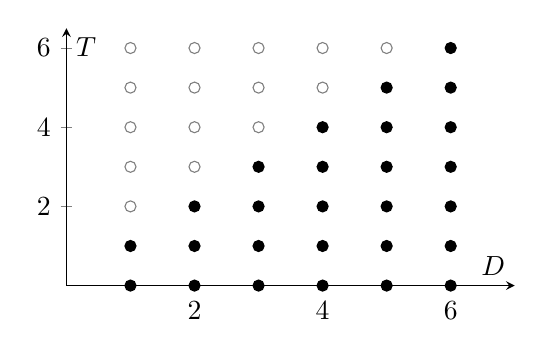
\begin{tikzpicture}
    \begin{axis}[
        axis lines = middle,
        xlabel = $D$,
        ylabel = $T$,
        width=0.6\textwidth,
        height=0.4\textwidth,
    ]

    \addplot [only marks, mark=*] table {
    1 0
    1 1
    2 0
    2 1
    2 2
    3 0
    3 1
    3 2
    3 3
    4 0
    4 1
    4 2
    4 3
    4 4
    5 0
    5 1
    5 2
    5 3
    5 4
    5 5
    6 0
    6 1
    6 2
    6 3
    6 4
    6 5
    6 6
    };

    \addplot [only marks, mark=o, color=gray] table {
    1 6
    1 5
    1 4
    1 3
    1 2
    2 6
    2 5
    2 4
    2 3
    3 6
    3 5
    3 4
    4 6
    4 5
    5 6
    };

    \addplot [draw=none, forget plot] coordinates {(7.0, 6.5)};
    \addplot [draw=none, forget plot] coordinates {(0, 0)};
    \end{axis}
    \end{tikzpicture}
    \caption{legge di $T|D$. I pallini pieni sono le combinazioni possibili.}
  \end{figure}

  Calcoliamo la probabilità richiesta mediante la definizione di probabilità condizionata (\ref{prob-condizionata}):
  $$P^{(D, T)}(n, k) = P^{T|D}(k|n) \cdot P^D(n) = \binom{n}{k} \ \frac 1 {2^n} \ \frac 1 6$$
  Da questo possiamo ottenere che:
  $$P^T(k)= \sum_{n=1}^{6} \frac{1}{6} \binom{n}{k} \frac{1}{2^n} \ \Ind_{[0,n]}(k)
  = \frac{1}{6} \sum\limits_{n = \max(1,k)}^6 \binom{n}{k} \frac{1}{2^n}$$
  Tramite la legge condizionata, molto più semplice, siamo riusciti a risalire alla legge di $T$.
\end{ese}

\subsubsection{Con due vettori aleatori}
Siano $X$ vettore aleatorio discreto in $\RR^n$ e $Y$ vettore aleatorio discreto in $\RR^m$. Definiamo $Q$ come:
$$Q(x, B) \coloneqq \begin{cases}
  \PP(Y \in B | X = x) & \text{per } x \in S_X \\
  \widetilde{Q}(B) & \text{per } x \not\in S_X
\end{cases}$$
$\widetilde Q(B)$ è un'arbitraria probabilità su $\Bc^m$.

Verifichiamo che $Q$ rispetti la definizione:
\begin{enumerate}
  \item $Q(\, \bigcdot \, , B)$ è misurabile in $x$: è costante su ${S_X}^C$ e al più numerabile su $S_X$.
  \item $Q(x, \, \bigcdot \,)$ è una probabilità: per la teoria se $x \in S_X$, per costruzione se $x \not\in S_X$.
  \item \Fixvmode \begin{align*}
    \int_E \Ind_A(x) \, Q(x, B) \, P^X(\dx) &= \sum_{x \in S_X} \Ind_A(x) \, Q(x, B) \, P^X(x) \\
    &= \sum_{x \in S_X} \Ind_A(x) \, \PP(Y \in B | X=x) \, P^X(x) \\
    &= \PP(X \in A, Y \in B)
  \end{align*}
  Notiamo che $\widetilde Q$ non ha ruolo nella sommatoria, in quanto è una probabilità assunta solo su eventi fuori dal supporto, i quali per definizione hanno probabilità nulla.
\end{enumerate}

\subsubsection{Caso rettangolare}
Sia $C \in A \times B$, con  $A, B \in \Bc$. Allora:
\begin{align*}
	\PP(X \in A, Y \in B) &= P^{(X, Y)}(A, B) \\
	&= \sum_{x \in A \cap S_X} \ \sum_{y \in B \cap S_Y} P^{(X, Y)}(x, y) \\
	&= \sum_{x \in A \cap S_X} \left[ \sum_{y \in B \cap S_Y} P^{(Y|X)}(y|x) \right] P^X(x) \\
	&= \sum_{x \in S_X} \Ind_A(x) \ \PP(Y \in B|X=x) \ \PP(X=x) \\
	&= \sum_{x \in S_X} \Ind_A(x) \, P^{Y|X}(B|x) \, P^X(x)
\end{align*}

\subsubsection{Caso generico}
Sia $C \in \Bc^2$ un generico boreliano. Allora:
\begin{align*}
  \PP((X, Y) \in C) &= P^{(X, Y)}(C) \\
  &= \sum_{(x, y) \in C} P^{(X, Y)}(x, y) & (\text{con }x \in S_X, \ y \in S_Y) \\
  &= \sum_{x \in S_X} \left[ \sum_{y: \, (x, y) \in C} P^{Y|X}(y|x) \right] \, P^X(x) \\
  &= \sum_{x \in S_X} \, \PP \left( (X, Y) \in C | X = x \right) \\
  &= \sum_{x \in S_X} \, \PP \left( (x, Y) \in C \right) &\text{(dipende solo da } Y \text{)}
\end{align*}

\subsection{Casi congiuntamente continui}
\subsubsection{Caso generico}
Sia $(X, Y)$ vettore aleatorio continuo in $\RR^n \times \RR^m$.
Denotiamo con $f_X$ e $f_Y$ le due densità marginali e con $f_{(X,Y)}$ la densità congiunta. Il supporto di $X$ si può scrivere come $S_X = \{ s \in \RR^n: f_X(s) > 0 \}$.

Definiamo $f_{Y|X}$ come:
$$f_{Y|X}(t) \coloneqq \begin{cases}
  \dfrac {f_{(X,Y)}(s, t)} {f_X(s)} & s \in S_X \\[8pt]
  \widetilde{f}(t) & s \not\in S_X
\end{cases}$$
Come prima, $\widetilde f(t)$ è un'arbitraria probabilità su $\RR^m$. \\
Si può dimostrare che $f_{Y|X}(t|s)$ è una densità di probabilità su $\RR^n$ per ogni $s$ fissato. La dimostrazione è lasciata come esercizio al lettore.\footnote{Ho sempre sognato di scriverlo, è un sogno che si avvera.}

\vskip\bigskipamount
\begin{prop}
  $$P^{Y|X}(B|s) = \int_B f_{Y|X}(t|s) \, \de t, \quad \text{ovvero }Y|X=s \sim f_{Y|X} (\, \bigcdot \, |s)$$
\end{prop}

Verifichiamo che $Q = P^{Y|X}$ rispetti la definizione.
Per le proprietà (1) e (2) si rimanda al caso discreto, poiché la dimostrazione è molto simile (per il punto (1) si sfrutta Fubini-Tonelli). La dimostrazione della (3) è la seguente:
\begin{align*}
  \int_{\RR^n} \Ind_A(s) \, Q(s, B) \, P^X(\de s)
  &= \int_{\RR^n} \Ind_A(s) \left[ \int_B f_{Y|X}(t|s) \de t \right] \, P^X(\de s) \\
  &= \int_A \int_B f_{(Y|X)}(t|s) \, f_X(s) \ \de s \, \de t \\
  &= \int_{A \cap S_X} \int_B \dfrac {f_{(X, Y)}(s,t)} {f_X(s)} \, f_X(s) \ \de s \, \de t \\
  &= \int_{A \cap S_X} \int_B f_{(X, Y)}(s,t) \ \de s \, \de t \\
  &= \PP(X \in A, Y \in B)
\end{align*}

\lezione{22}{25.05.2017}
\begin{prop}
  Sia $(X,Y)$ vettore continuo in $\RR^n \times \RR^m$.
  Allora $Y|X=s$ è un vettore continuo con densità:
  $$f_{Y|X}(t | s) = \frac{f_{(X,Y)}(s,t)}{f_X (s)} \quad \forall s \in S_X$$
  \end{prop}

\begin{prop}
  Sia $(X,Y)$ vettore aleatorio in $\RR^n \times \RR^m$; inoltre, $X$ è continua con densità $f_X$ e $Y|X = s$ è pure continua con densità $f_{Y|X}(\, \bigcdot \, | s) \; \forall s \in S_X$.
  Allora $(X,Y)$ è continuo con densità:
  $$f_{(X,Y)} (s,t) = f_X(s) f_{(Y|X)}(t|s) \quad \forall s \in \RR^n, \enspace \forall t \in \RR^m$$
\end{prop}

\begin{dimo}\belowdisplayskip=-21pt
  Prendiamo due eventi $A$ e $B$ sulle rispettive $\sigma$-algebre e riscriviamone la probabilità\footnote{Cosa ti ha fatto pensare che questa dimostrazione sarà diversa dalle 10 precedenti?}:
  \begin{align*}
    \PP(X \in A, Y \in B) &= P^{(X,Y)} (A \times B) \\
    &= \int_{\RR^m} \Ind_A(X) \, Q_{(X,B)} P^X(\dx) \\
    &= \int_{A} \left( \int_{B} f_{Y|X} (t|s) \de t \right) f_X(s) \, \de s \\
    &= \int_{A \times B} f_X(s) \, f_{Y|X} (t|s) \, \de s\,  \de t &\hspace{12em}
  \end{align*}\qedhere
\end{dimo}

\subsubsection{Caso gaussiano per una coppia di variabili}

In due dimensioni:
$$\begin{bmatrix}X \\ Y\end{bmatrix} \sim \Nc(\mu, C) = \Nc \left( \begin{bmatrix}\mu_X \\ \mu_Y\end{bmatrix}, \begin{bmatrix}\sigma_X^2 & \rho\sigma_X\sigma_Y \\ \rho\sigma_X\sigma_Y & \sigma_Y^2 \end{bmatrix} \right)$$

Che legge ha $Y|X = s$?
\begin{itemize}
  \item Nel caso in cui $\sigma_X = 0$, si ha $X \sim \Nc(\mu_X, 0) = \delta_{\mu_X} \implies \PP\left(X = \mu_X\right) = 1$\\
    $\implies Y|X = \mu_X \sim Y \sim \Nc(\mu_Y, \sigma_Y^2)$

  \item Nel caso in cui $\sigma_X > 0$, si ha $Y|X = s \sim \Nc(m(s), q^2)$, dove $m(s)$ indica la media (forma compatta per $\EE[Y|X = s]$). In particolare:
    $$m(s) = \mu_Y + \frac{Cov(X,Y)}{Var(X)}(s-\mu_X) = \mu_Y + \rho \frac{\sigma_Y}{\sigma_X}(s-\mu_X)$$
    $$q^2 = Var(Y|X=s)  = Var(Y) - \frac{Cov(X,Y)}{Var(X)} = \sigma_Y^2(1-\rho^2)$$
\end{itemize}

\begin{oss}
  \Fixvmode
  \begin{enumerate}
    \item $y = m(x)$ è la retta di regressione lineare (oggetto sviscerato in statistica).
    \item $q^2$ non dipende da $s$.
    \item Casi notevoli:
    \begin{enumerate}
      \item $\rho = 0 \iff X \indep Y \implies Y|X = s \sim \Nc(\mu_Y, \sigma_Y^2)$;
      \item $\abs{\rho} = 1 \iff Y = AX+b \implies Y|X = s \sim \Nc(\mu_Y + \rho\frac{\sigma_Y}{\sigma_X} (s - \mu_X), 0)$.

      Questo è il caso di totale dipendenza, opposto al punto (1);
      \item $\sigma_Y^2 = 0 \iff Y \sim \Nc(\mu_Y, 0) \implies Y|X = s \sim \Nc(\mu_Y, 0)$;
      \item $q^2 \leq \sigma_Y^2$ e solo nel caso $X \indep Y$ vale l'uguaglianza: $q^2 = \sigma_Y^2$;
      \item $Y|X = s \sim \Nc \enspace \forall s$.
    \end{enumerate}
  \end{enumerate}
\end{oss}

\subsubsection{Caso gaussiano per una coppia di vettori}

\begin{prop}
  Siano $X \sim \Nc(\mu_X, C_X)$ $n$-dimensionale e $Y \sim \Nc(\mu_Y, C_Y)$ $m$-dimensionale. \\*
  Allora:
  $$\begin{bmatrix}X \\ Y \end{bmatrix} \sim \Nc \left(\begin{bmatrix}\mu_X \\ \mu_Y \end{bmatrix}, \begin{bmatrix}C_X & C_{XY} \\ C_{YX} & C_Y \end{bmatrix}\right)$$
  % $\mu_X = \EE[X]$, $\mu_Y = \EE[Y]$, $Var(X) = C_X$,  $Var(Y) = C_Y$
  % ↑ Non serve davvero tutta sta roba...

  Inoltre vale ovviamente $C_{XY} = C_{YX}^T$.
\end{prop}

\medskip
\begin{prop}
  Se $C_X$ è invertibile, ovvero $\det(C_X) > 0$, allora:
  \begin{itemize}
    \item $Y|X=s \sim \Nc(m(s), Q)$;
    \item $m(s) = \EE[Y|X=s] = \mu_Y + C_{YX} C_X^{-1} (s-\mu_X)$;
    \item $Q = Var(Y|X=s) = C_Y - C_{YX}C_X^{-1}C_{XY}$.
  \end{itemize}
\end{prop}

\subsection{Caso misto}
Sia $(X,Y)$ vettore aleatorio in $\RR^{n+m}$. \\
Siano inoltre $X$ VA discreta di densità $P_X$ e $Y|X = s$ continua di densità \\* $f_{Y|X} (\, \bigcdot \,| s) \ \forall s \in S_X$.\\*
Avendo una componente continua e una discreta, fissiamo una delle due e calcoliamo l'altra:
\begin{align*}
	\PP(X \in A, Y \in B) &= \PP^{(X,Y)} (A \times B) \\
	&= \int_{\RR^n} \Ind_A (s) \, Q(s,B) P^X (\de s) \\
	&=\sum\limits_{s \in S_X} \Ind_A (s) \left( \int_{B}  f_{Y|X} (t|s) \, \de t \, P^X(s) \right) \\
	&= \sum\limits_{s \in A \cap S_X} \left(\int_{B} f_{Y|X} (t|s) P^X(s) \, \de t \right)
\end{align*}

Che legge ha $Y$? Per scoprirlo si ponga $A = \RR^n$, da cui discende che $(X \in \RR^n) = \Omega$. Applichiamo ora la formula di sopra:
\begin{align*}
	P(Y \in B) &= \sum\limits_{s \in S_X} \left( \int_{B} f_{Y|X} (t|s) P^X (s) \, \de t \right) &\\
	&= \int_{B} \left( \sum\limits_{s \in S_X} f_{Y|X} (t|s) P^X (s) \right) \de t &\text{(per Fubini-Tonelli)}\\
	&= \int_{B} f_Y(t) \, \de t &
\end{align*}
Quindi $Y$ è un vettore continuo con densità $f_Y$.

\cleardoublepage
